\documentclass[manuscript,screen]{acmart}
\AtBeginDocument{%
  \providecommand\BibTeX{{%
    Bib\TeX}}}

\setcopyright{acmlicensed}
\copyrightyear{2025}
\acmYear{2025}
\acmDOI{XXXXXXX.XXXXXXX}
\acmConference[Conference 'XX]{}{June 03--05,
  2018}{Woodstock, NY}
\acmISBN{978-1-4503-XXXX-X/2018/06}






\usepackage[tight,footnotesize]{subfigure}
\usepackage{tikz}
\usepackage{color, pifont, comment}
\usepackage{xspace}
\usepackage{algorithm}
\usepackage{algpseudocode}
\usepackage{enumerate}
\usepackage{enumitem}

\usepackage[export]{adjustbox}
\usepackage{stmaryrd}
\usepackage{colortbl}
\usepackage{xurl}
\usepackage[compact]{titlesec}
\usepackage[subtle,tracking=normal]{savetrees}
\usepackage{fontawesome5}
\usepackage{eqparbox}

\usepackage{pifont, comment}
\usepackage{xspace}
\usepackage{upquote}
\usepackage{listings}
\usepackage{xcolor}


\usepackage{cases}

\usepackage{caption}
\usepackage{multirow}
\usepackage{tabularx}

\newcommand{\ie}{{\it i.e.,}\xspace}
\newcommand{\eg}{{\it e.g.,}\xspace}
\newcommand{\etc}{{\it etc.}\xspace}
\newcommand{\vs}{{\it vs.}\xspace}
\newcommand{\etal}{{\it et al.}\xspace}
\newcommand{\descr}[1]{\vspace{.05in} \noindent\textbf{#1}}
\newcommand{\tilda}{\raise.17ex\hbox{$\scriptstyle\mathtt{\sim}$}}
\newcommand{\tool}{{AutoLike}}
\newcommand{\autolike}{{AutoLike}}
\newcommand{\rs}{{RS}}
\newcommand{\recsys}{{recommendation system}}
\newcommand{\fyp}{{FYP}}
\newcommand{\si}{{$SI$}} %
\newcommand{\autolikedatasetone}{AUTOLIKE-D1} 
\newcommand{\autolikedatasettwo}{AUTOLIKE-D2}
\newcommand{\TODO}[1]{\textcolor{red}{#1}}

\begin{document}

\title{\autolike{}: Auditing Social Media Recommendations through User  Interactions}

\author{Hieu Le}
\authornote{This work was primarily completed  during the author's graduate studies at the University of California, Irvine.}
\email{levanhieu@gmail.com}
\affiliation{%
  \institution{University of California, Irvine}
  \city{Irvine}
  \state{California}
  \country{USA}
}

\author{Salma Elmalaki}
\email{salma.elmalaki@uci.edu}
\affiliation{%
  \institution{University of California, Irvine}
  \city{Irvine}
  \state{California}
  \country{USA}
  }


\author{Zubair Shafiq}
\email{zubair@ucdavis.edu}
\affiliation{%
  \institution{University of California, Davis}
  \city{Davis}
  \state{California}
  \country{USA}
}

\author{Athina Markopoulou}
\email{athina@uci.edu}
\affiliation{%
  \institution{University of California, Irvine}
  \city{Irvine}
  \state{California}
  \country{USA}
 }


\renewcommand{\shortauthors}{Le et al.}

\begin{abstract}
Modern social media platforms, such as TikTok, Facebook, and YouTube, rely on recommendation systems to personalize content for users based on user interactions with endless streams of content, such as ``For You'' pages. However, these complex algorithms can inadvertently deliver problematic content related to self-harm, mental health, and eating disorders. %
We introduce AutoLike, a framework to audit recommendation systems in social media platforms for topics of interest and their sentiments. To automate the process, we formulate the problem as a reinforcement learning problem. AutoLike drives the recommendation system to serve a particular type of content through interactions (e.g., liking).
We apply the AutoLike framework to the TikTok platform as a case study. We evaluate how well AutoLike identifies TikTok content automatically across nine topics of interest; and conduct eight experiments to demonstrate how well it drives TikTok's recommendation system towards particular topics and sentiments. AutoLike has the potential to assist regulators in auditing recommendation systems for problematic content. \textbf{(Warning: This paper contains qualitative examples that may be viewed as offensive or harmful.)}
\end{abstract}

\begin{CCSXML}
<ccs2012>
 <concept>
  <concept_id>00000000.0000000.0000000</concept_id>
  <concept_desc>Do Not Use This Code, Generate the Correct Terms for Your Paper</concept_desc>
  <concept_significance>500</concept_significance>
 </concept>
 <concept>
  <concept_id>00000000.00000000.00000000</concept_id>
  <concept_desc>Do Not Use This Code, Generate the Correct Terms for Your Paper</concept_desc>
  <concept_significance>300</concept_significance>
 </concept>
 <concept>
  <concept_id>00000000.00000000.00000000</concept_id>
  <concept_desc>Do Not Use This Code, Generate the Correct Terms for Your Paper</concept_desc>
  <concept_significance>100</concept_significance>
 </concept>
 <concept>
  <concept_id>00000000.00000000.00000000</concept_id>
  <concept_desc>Do Not Use This Code, Generate the Correct Terms for Your Paper</concept_desc>
  <concept_significance>100</concept_significance>
 </concept>
</ccs2012>
\end{CCSXML}


\keywords{Social Media, Recommendations, Algorithmic Auditing}


\maketitle

\section{Introduction}
\label{sec:introduction}
The business processes of organizations are experiencing ever-increasing complexity due to the large amount of data, high number of users, and high-tech devices involved \cite{martin2021pmopportunitieschallenges, beerepoot2023biggestbpmproblems}. This complexity may cause business processes to deviate from normal control flow due to unforeseen and disruptive anomalies \cite{adams2023proceddsriftdetection}. These control-flow anomalies manifest as unknown, skipped, and wrongly-ordered activities in the traces of event logs monitored from the execution of business processes \cite{ko2023adsystematicreview}. For the sake of clarity, let us consider an illustrative example of such anomalies. Figure \ref{FP_ANOMALIES} shows a so-called event log footprint, which captures the control flow relations of four activities of a hypothetical event log. In particular, this footprint captures the control-flow relations between activities \texttt{a}, \texttt{b}, \texttt{c} and \texttt{d}. These are the causal ($\rightarrow$) relation, concurrent ($\parallel$) relation, and other ($\#$) relations such as exclusivity or non-local dependency \cite{aalst2022pmhandbook}. In addition, on the right are six traces, of which five exhibit skipped, wrongly-ordered and unknown control-flow anomalies. For example, $\langle$\texttt{a b d}$\rangle$ has a skipped activity, which is \texttt{c}. Because of this skipped activity, the control-flow relation \texttt{b}$\,\#\,$\texttt{d} is violated, since \texttt{d} directly follows \texttt{b} in the anomalous trace.
\begin{figure}[!t]
\centering
\includegraphics[width=0.9\columnwidth]{images/FP_ANOMALIES.png}
\caption{An example event log footprint with six traces, of which five exhibit control-flow anomalies.}
\label{FP_ANOMALIES}
\end{figure}

\subsection{Control-flow anomaly detection}
Control-flow anomaly detection techniques aim to characterize the normal control flow from event logs and verify whether these deviations occur in new event logs \cite{ko2023adsystematicreview}. To develop control-flow anomaly detection techniques, \revision{process mining} has seen widespread adoption owing to process discovery and \revision{conformance checking}. On the one hand, process discovery is a set of algorithms that encode control-flow relations as a set of model elements and constraints according to a given modeling formalism \cite{aalst2022pmhandbook}; hereafter, we refer to the Petri net, a widespread modeling formalism. On the other hand, \revision{conformance checking} is an explainable set of algorithms that allows linking any deviations with the reference Petri net and providing the fitness measure, namely a measure of how much the Petri net fits the new event log \cite{aalst2022pmhandbook}. Many control-flow anomaly detection techniques based on \revision{conformance checking} (hereafter, \revision{conformance checking}-based techniques) use the fitness measure to determine whether an event log is anomalous \cite{bezerra2009pmad, bezerra2013adlogspais, myers2018icsadpm, pecchia2020applicationfailuresanalysispm}. 

The scientific literature also includes many \revision{conformance checking}-independent techniques for control-flow anomaly detection that combine specific types of trace encodings with machine/deep learning \cite{ko2023adsystematicreview, tavares2023pmtraceencoding}. Whereas these techniques are very effective, their explainability is challenging due to both the type of trace encoding employed and the machine/deep learning model used \cite{rawal2022trustworthyaiadvances,li2023explainablead}. Hence, in the following, we focus on the shortcomings of \revision{conformance checking}-based techniques to investigate whether it is possible to support the development of competitive control-flow anomaly detection techniques while maintaining the explainable nature of \revision{conformance checking}.
\begin{figure}[!t]
\centering
\includegraphics[width=\columnwidth]{images/HIGH_LEVEL_VIEW.png}
\caption{A high-level view of the proposed framework for combining \revision{process mining}-based feature extraction with dimensionality reduction for control-flow anomaly detection.}
\label{HIGH_LEVEL_VIEW}
\end{figure}

\subsection{Shortcomings of \revision{conformance checking}-based techniques}
Unfortunately, the detection effectiveness of \revision{conformance checking}-based techniques is affected by noisy data and low-quality Petri nets, which may be due to human errors in the modeling process or representational bias of process discovery algorithms \cite{bezerra2013adlogspais, pecchia2020applicationfailuresanalysispm, aalst2016pm}. Specifically, on the one hand, noisy data may introduce infrequent and deceptive control-flow relations that may result in inconsistent fitness measures, whereas, on the other hand, checking event logs against a low-quality Petri net could lead to an unreliable distribution of fitness measures. Nonetheless, such Petri nets can still be used as references to obtain insightful information for \revision{process mining}-based feature extraction, supporting the development of competitive and explainable \revision{conformance checking}-based techniques for control-flow anomaly detection despite the problems above. For example, a few works outline that token-based \revision{conformance checking} can be used for \revision{process mining}-based feature extraction to build tabular data and develop effective \revision{conformance checking}-based techniques for control-flow anomaly detection \cite{singh2022lapmsh, debenedictis2023dtadiiot}. However, to the best of our knowledge, the scientific literature lacks a structured proposal for \revision{process mining}-based feature extraction using the state-of-the-art \revision{conformance checking} variant, namely alignment-based \revision{conformance checking}.

\subsection{Contributions}
We propose a novel \revision{process mining}-based feature extraction approach with alignment-based \revision{conformance checking}. This variant aligns the deviating control flow with a reference Petri net; the resulting alignment can be inspected to extract additional statistics such as the number of times a given activity caused mismatches \cite{aalst2022pmhandbook}. We integrate this approach into a flexible and explainable framework for developing techniques for control-flow anomaly detection. The framework combines \revision{process mining}-based feature extraction and dimensionality reduction to handle high-dimensional feature sets, achieve detection effectiveness, and support explainability. Notably, in addition to our proposed \revision{process mining}-based feature extraction approach, the framework allows employing other approaches, enabling a fair comparison of multiple \revision{conformance checking}-based and \revision{conformance checking}-independent techniques for control-flow anomaly detection. Figure \ref{HIGH_LEVEL_VIEW} shows a high-level view of the framework. Business processes are monitored, and event logs obtained from the database of information systems. Subsequently, \revision{process mining}-based feature extraction is applied to these event logs and tabular data input to dimensionality reduction to identify control-flow anomalies. We apply several \revision{conformance checking}-based and \revision{conformance checking}-independent framework techniques to publicly available datasets, simulated data of a case study from railways, and real-world data of a case study from healthcare. We show that the framework techniques implementing our approach outperform the baseline \revision{conformance checking}-based techniques while maintaining the explainable nature of \revision{conformance checking}.

In summary, the contributions of this paper are as follows.
\begin{itemize}
    \item{
        A novel \revision{process mining}-based feature extraction approach to support the development of competitive and explainable \revision{conformance checking}-based techniques for control-flow anomaly detection.
    }
    \item{
        A flexible and explainable framework for developing techniques for control-flow anomaly detection using \revision{process mining}-based feature extraction and dimensionality reduction.
    }
    \item{
        Application to synthetic and real-world datasets of several \revision{conformance checking}-based and \revision{conformance checking}-independent framework techniques, evaluating their detection effectiveness and explainability.
    }
\end{itemize}

The rest of the paper is organized as follows.
\begin{itemize}
    \item Section \ref{sec:related_work} reviews the existing techniques for control-flow anomaly detection, categorizing them into \revision{conformance checking}-based and \revision{conformance checking}-independent techniques.
    \item Section \ref{sec:abccfe} provides the preliminaries of \revision{process mining} to establish the notation used throughout the paper, and delves into the details of the proposed \revision{process mining}-based feature extraction approach with alignment-based \revision{conformance checking}.
    \item Section \ref{sec:framework} describes the framework for developing \revision{conformance checking}-based and \revision{conformance checking}-independent techniques for control-flow anomaly detection that combine \revision{process mining}-based feature extraction and dimensionality reduction.
    \item Section \ref{sec:evaluation} presents the experiments conducted with multiple framework and baseline techniques using data from publicly available datasets and case studies.
    \item Section \ref{sec:conclusions} draws the conclusions and presents future work.
\end{itemize}
\begin{figure*}[ht]
    \centering
    \includegraphics[width=\textwidth, trim=79 280 93 123, clip]{figures/framework_img.pdf}
    \caption{The pipeline of the \ENDow{} framework 
    %where each component is specified in a given configuration. 
    which yields a downstream task score and a WER score of the transcript set input to the task. The pipeline is executed for several severeties of noising and types of cleaning techniques. %Acoustic noising is applied at $k$ intensities, providing $k+1$ audio versions (including the non-noised version), eventually producing $k+2$ transcript versions (including the source transcript). Applying transcript cleaning reveals the effect of \textit{types} of noise. 
    Resulting scores are plotted on a graph for the analyses, as in, e.g., \autoref{fig_cleaning_graphs}.}
    %The pipeline is executed on $k+1$ intensities of acoustic noising (including the non-noised version), producing $k+2$ scores for the downstream task (including execution on the source transcripts). This process eventually describes the effect of the \textit{intensity} of transcript noise on the downstream task. The process is repeated for $m$ cleaning techniques ($m+1$ when including no cleaning), to analyze the benefit of a cleaning approach and the effect of the \textit{types} of transcript noise.}
    \label{fig_framework}
\end{figure*}
\chapter{Implementation}{\label{ch:implementation}}
In this chapter, we present the implementation of the final product. We start by discussing how the four steps introduced in \hyperref[ch:high_level_approach]{chapter \ref*{ch:high_level_approach}} are integrated. We then outline the main system components of our score follower, presenting each as an independent, self-contained module. We then combine this into an overall system architecture and finally introduce the open-source score renderer used to display the score and evaluate the score follower.       

% \section{Aims and Requirements}
% The overall aim of the score follower was to 


\section{Score Follower Framework Details}
Our score follower conforms to the high-level framework presented in \hyperref[section:score_follower_framework]{section \ref*{section:score_follower_framework}}. In step 1, two score features are extracted from a MIDI file (see \hyperref[subsection:midi]{subsection \ref*{subsection:midi}}), namely MIDI note numbers\footnote{\href{https://inspiredacoustics.com/en/MIDI_note_numbers_and_center_frequencies}{https://inspiredacoustics.com/en/MIDI\_note\_numbers\_and\_center\_frequencies}} (corresponding to pitch) and note onsets (corresponding to duration). In step 2, the audio is streamed (whether from a file or into a microphone) and audioframes that exceed some predefined energy threshold are extracted. Here, audioframes are groups of contiguous audio samples, whose length can be specified by the argument \verb|frame_length|, usually between 800 and 2000 samples. The period between consecutive audioframes can also be defined by the argument \verb|hop_length|, typically between 2000 and 5000 audio samples. In step 3, score following is performed via a `Windowed' Viterbi algorithm (see  \hyperref[subsection:adjusting_viterbi]{subsection \ref*{subsection:adjusting_viterbi}}) which uses the Gaussian Process (GP) log marginal likelihoods (LMLs) for emission probabilities (see \hyperref[section:state_duration_model]{section \ref*{section:state_duration_model}}) and a state duration model for transition probabilities (see \hyperref[section:state_duration_model]{section \ref*{section:state_duration_model}}). Finally, in step 4 we render our results using an adapted version of the open source user interface, \textit{Flippy Qualitative Testbench}.

\section{Following Modes}
Two modes are available to the user: Pre-recorded Mode and Live Mode. The former requires a pre-recorded $\verb|.wav|$ file, whereas the latter takes an input stream of audio via the device's microphone. Note that both modes are still forms of score following, as opposed to score alignment, since in each mode we receive audioframes at the sampling rate, not all at once.\\

Live Mode offers a practical example of a score follower, displaying a score and position marker which a musician can read off while playing. However, this mode is not suitable for evaluation because the input and results cannot be easily replicated. Even ignoring repeatability, Live Mode is not suitable for one-off testing since a musician using this application may be influenced by the movement of the marker. For instance, the performer may speed up if the score follower `gets ahead' or slow down if the position marker lags or `gets lost'. To avoid this, we use Pre-recorded Mode when evaluating the performance of our score follower. Furthermore, Pre-recorded Mode offers the advantage of testing away from the music room, providing the opportunity to evaluate a variety of recordings available online. 

\section{System Architecture}
Our guiding principle for development was to build modular code in order to create a streamlined system where each component performs a specific task independently. This structure facilitates easy testing and debugging. \hyperref[fig:black_box]{Figure \ref*{fig:black_box}} presents a high-level architecture diagram, where each black box abstracts a key component of the score follower. When operating in Pre-recorded Mode, there is the option to stream the recording during run-time, which outputs to the device's speakers (as indicated by the dashed lines).

\begin{figure}[H]
    \centering
    \includegraphics[width=1\textwidth]{figs/Part_4_Implementation_And_Results/black_box.png}
    \caption{Abstracted system architecture diagram displaying inputs in grey, the 4 main components of the score follower in black and the outputs in green.}
    \label{fig:black_box}
\end{figure}

\subsection{Score Preprocessor}
The architecture for the Score Preprocesor is given in \hyperref[fig:score_preprocessor]{Figure \ref*{fig:score_preprocessor}}. First, MIDI note number and note onset times are extracted from each MIDI event. Simultaneous notes can be gathered into states and returned as a time-sorted list of lists called \verb|score|, where each element of the outer list is a list of simultaneous note onsets. Similarly, a list of note durations calculated as the time difference between consecutive states is returned as \verb|times_to_next|. Finally, all covariance matrices are precalculated and stored in a dictionary, where the key of the dictionary is determined by the notes present. This is because the distribution of notes and chords in a score is not random: notes tend to belong to a home \gls{key} and melodies tend to be repeated or related (similar to subject fields in speech processing). Therefore, states tend to be reused often, allowing us to achieve amortised time and space savings (by avoiding repeated calculation of the same covariance matrices). 

\begin{figure}[H]
    \centering
    \includegraphics[width=1\textwidth]{figs/Part_3_Implementation/Stage_2_Alignment/score_preprocessor.png}
    \caption{System architecture diagram representing the Score Preprocessor with inputs in grey, processes in blue and objects in yellow.}
    \label{fig:score_preprocessor}
\end{figure}


\subsection{Audio Preprocessor}
The architecture for the Audio Preprocessor is illustrated in \hyperref[fig:audio_preprocessor]{Figure \ref*{fig:audio_preprocessor}}. In Pre-recorded Mode, the Slicer receives a $\verb|.wav|$ file and returns audioframes separated by the \verb|hop_length|. These audioframes are periodically added to a multiprocessing queue, \verb|AudioFramesQueue|, to simulate real-time score following. In Live Mode, we use the python module \verb|sounddevice| to receive a stream of audio, using a periodic callback function to place audioframes on \verb|AudioFramesQueue|. 

\begin{figure}[H]
    \centering
    \includegraphics[width=1\textwidth]{figs/Part_4_Implementation_And_Results/audio_preprocessor.png}
    \caption{System architecture diagram representing the Audio Preprocessor with inputs in grey, processes in blue and objects in yellow.}
    \label{fig:audio_preprocessor}
\end{figure}

\subsection{Follower and Backend}
The joint Follower and Backend architecture diagram is shown in \hyperref[fig:follwer_and_backend]{Figure \ref*{fig:follwer_and_backend}}. The Viterbi Follower (detailed in \hyperref[subsection:adjusting_viterbi]{section \ref*{subsection:adjusting_viterbi}}) calculates the most probable state in the score, given audioframes continually taken from \verb|AudioFramesQueue|. These states are placed on another multiprocessing queue, the \verb|FollowerOutputQueue|, for the Backend to process and send. This prevents any bottle-necking occurring at the Follower stage. The Backend first sets up a UDP connection and then reads off values from \verb|FollowerOutputQueue|, sending them via UDP packets to the score renderer.

\begin{figure}[H]
    \centering
    \includegraphics[width=1\textwidth]{figs/Part_4_Implementation_And_Results/follower_and_backend.png}
    \caption{System architecture diagram representing the Follower and Backend processes with processes in blue, objects in yellow and outputs in green.}
    \label{fig:follwer_and_backend}
\end{figure}

\subsection{Player}
In Pre-recorded Mode, the Player sets up a new process and begins streaming the recording once the Follower process begins. This provides a baseline for testing purposes, as a trained musician can observe the score position marker and judge how well it matches the music. 

\subsection{Overall System Architecture}
The overall system architecture is presented in \hyperref[fig:overall_system_architecture]{Figure \ref*{fig:overall_system_architecture}}. Since the Follower runs a real-time, time sensitive process, parallelism is employed to reduce the total system latency. We use two \verb|multiprocessing| queues\footnote{\href{https://docs.python.org/3/library/multiprocessing.html}{https://docs.python.org/3/library/multiprocessing.html}} to avoid bottle-necking, which allows us to run 4 concurrent processes (Audio Preprocessor, Follower, Backend, and Audio Player). Hence, this architecture allows the components to run independently of one another to avoid blocking. Furthermore, this allows the system to take advantage of the multiple cores and high computational power offered by most modern machines.  

\begin{figure}[H]
    \centering
    \includegraphics[width=1\textwidth]{figs/Part_4_Implementation_And_Results/overall_score_follower_2.png}
    \caption{System architecture diagram representing the overall score follower running in Pre-recorded mode, with inputs in grey, processes in blue, objects in yellow and outputs in green.}
    \label{fig:overall_system_architecture}
\end{figure}


\section{Rendering Results}{\label{section:renderer}}
To visualise the results of our score follower, we adapted an open source tool for testing different score followers.\footnote{\href{https://github.com/flippy-fyp/flippy-qualitative-testbench/blob/main/README.md}{https://github.com/flippy-fyp/flippy-qualitative-testbench/blob/main/README.md}} \hyperref[fig:flippy_example]{Figure \ref*{fig:flippy_example}} shows the user interface of the score position renderer, where the green bar indicates score position. 

\begin{figure}[H]
    \centering
    \includegraphics{figs/Part_4_Implementation_And_Results/example_renderer.png}
    \caption{Screenshot of the score renderer user interface which displays a score (here we show a keyboard arrangement of \textit{O Haupt voll Blut und Wunden} by Bach). The green marker represents the score follower position.}
    \label{fig:flippy_example}
\end{figure}



\definecolor{darkgreen}{rgb}{0.0, 0.5, 0.0}
\definecolor{violet}{rgb}{0.56, 0.0, 1.0}
\section{Evaluation}
We apply our methodology to derive counterfactual policies for various MDPs, addressing three main research questions: (1) how does our policy's performance compare to the Gumbel-max SCM approach; (2) how do the counterfactual stability and monotonicity assumptions impact the probability bounds; and (3) how fast is our approach compared with the Gumbel-max SCM method?

\begin{figure*}
    \centering
    %
    \resizebox{0.6\textwidth}{!}{
        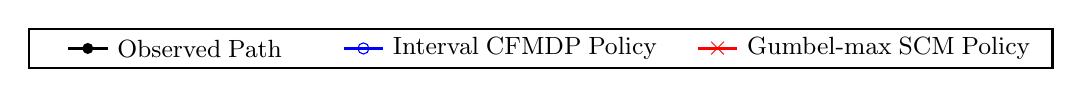
\begin{tikzpicture}[scale=1.0, every node/.style={scale=1.0}]
            \draw[thick, black] (-3, -0.25) rectangle (10, 0.25);
            %
            \draw[black, line width=1pt] (-2.5, 0.0) -- (-2,0.0);
            \fill[black] (-2.25,0.0) circle (2pt); %
            \node[right] at (-2,0.0) {\small Observed Path};
            
            %
            \draw[blue, line width=1pt] (1.0,0.0) -- (1.5,0.0);
            \node[draw=blue, circle, minimum size=4pt, inner sep=0pt] at (1.25,0.0) {}; %
            \node[right] at (1.5,0.0) {\small Interval CFMDP Policy};
            
            %
            \draw[red, line width=1pt] (5.5,0) -- (6,0);
            \node[red] at (5.75,0) {$\boldsymbol{\times}$}; %
            \node[right] at (6,0) {\small Gumbel-max SCM Policy};
        \end{tikzpicture}
    }\\
    %
    \subfigure[\footnotesize Lowest cumulative reward: Interval CFMDP ($312$), Gumbel-max SCM ($312$)]{%
        \resizebox{0.76\columnwidth}{!}{
             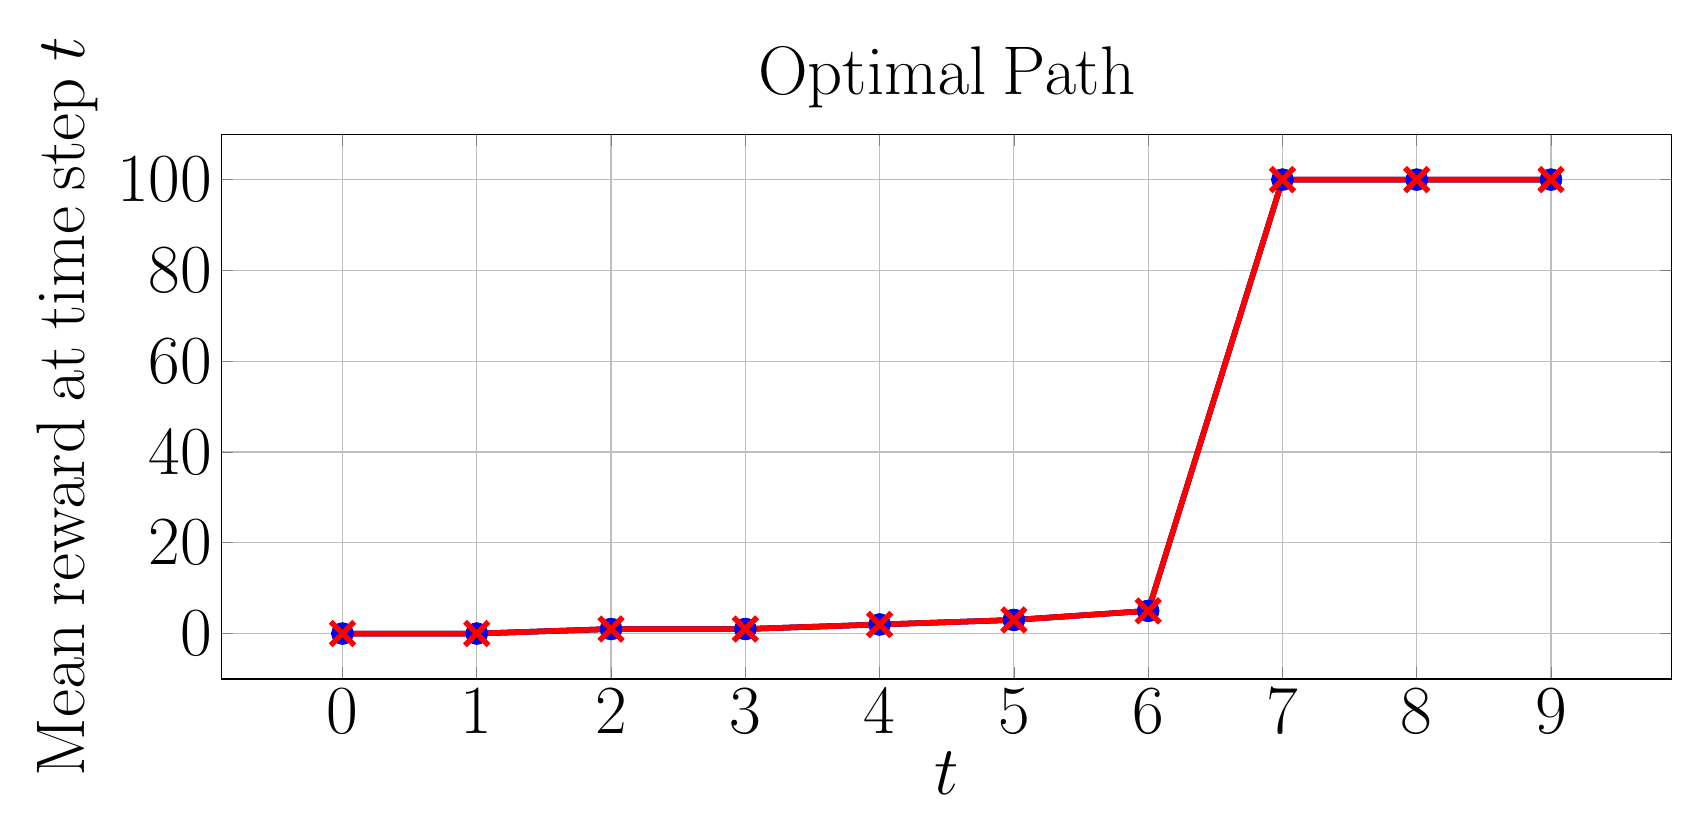
\begin{tikzpicture}
                \begin{axis}[
                    xlabel={$t$},
                    ylabel={Mean reward at time step $t$},
                    title={Optimal Path},
                    grid=both,
                    width=20cm, height=8.5cm,
                    every axis/.style={font=\Huge},
                    %
                ]
                \addplot[
                    color=black, %
                    mark=*, %
                    line width=2pt,
                    mark size=3pt,
                    error bars/.cd,
                    y dir=both, %
                    y explicit, %
                    error bar style={line width=1pt,solid},
                    error mark options={line width=1pt,mark size=4pt,rotate=90}
                ]
                coordinates {
                    (0, 0.0)  +- (0, 0.0)
                    (1, 0.0)  +- (0, 0.0) 
                    (2, 1.0)  +- (0, 0.0) 
                    (3, 1.0)  +- (0, 0.0)
                    (4, 2.0)  +- (0, 0.0)
                    (5, 3.0) +- (0, 0.0)
                    (6, 5.0) +- (0, 0.0)
                    (7, 100.0) +- (0, 0.0)
                    (8, 100.0) +- (0, 0.0)
                    (9, 100.0) +- (0, 0.0)
                };
                %
                \addplot[
                    color=blue, %
                    mark=o, %
                    line width=2pt,
                    mark size=3pt,
                    error bars/.cd,
                    y dir=both, %
                    y explicit, %
                    error bar style={line width=1pt,solid},
                    error mark options={line width=1pt,mark size=4pt,rotate=90}
                ]
                 coordinates {
                    (0, 0.0)  +- (0, 0.0)
                    (1, 0.0)  +- (0, 0.0) 
                    (2, 1.0)  +- (0, 0.0) 
                    (3, 1.0)  +- (0, 0.0)
                    (4, 2.0)  +- (0, 0.0)
                    (5, 3.0) +- (0, 0.0)
                    (6, 5.0) +- (0, 0.0)
                    (7, 100.0) +- (0, 0.0)
                    (8, 100.0) +- (0, 0.0)
                    (9, 100.0) +- (0, 0.0)
                };
                %
                \addplot[
                    color=red, %
                    mark=x, %
                    line width=2pt,
                    mark size=6pt,
                    error bars/.cd,
                    y dir=both, %
                    y explicit, %
                    error bar style={line width=1pt,solid},
                    error mark options={line width=1pt,mark size=4pt,rotate=90}
                ]
                coordinates {
                    (0, 0.0)  +- (0, 0.0)
                    (1, 0.0)  +- (0, 0.0) 
                    (2, 1.0)  +- (0, 0.0) 
                    (3, 1.0)  +- (0, 0.0)
                    (4, 2.0)  +- (0, 0.0)
                    (5, 3.0) +- (0, 0.0)
                    (6, 5.0) +- (0, 0.0)
                    (7, 100.0) +- (0, 0.0)
                    (8, 100.0) +- (0, 0.0)
                    (9, 100.0) +- (0, 0.0)
                };
                \end{axis}
            \end{tikzpicture}
         }
    }
    \hspace{1cm}
    \subfigure[\footnotesize Lowest cumulative reward: Interval CFMDP ($19$), Gumbel-max SCM ($-88$)]{%
         \resizebox{0.76\columnwidth}{!}{
            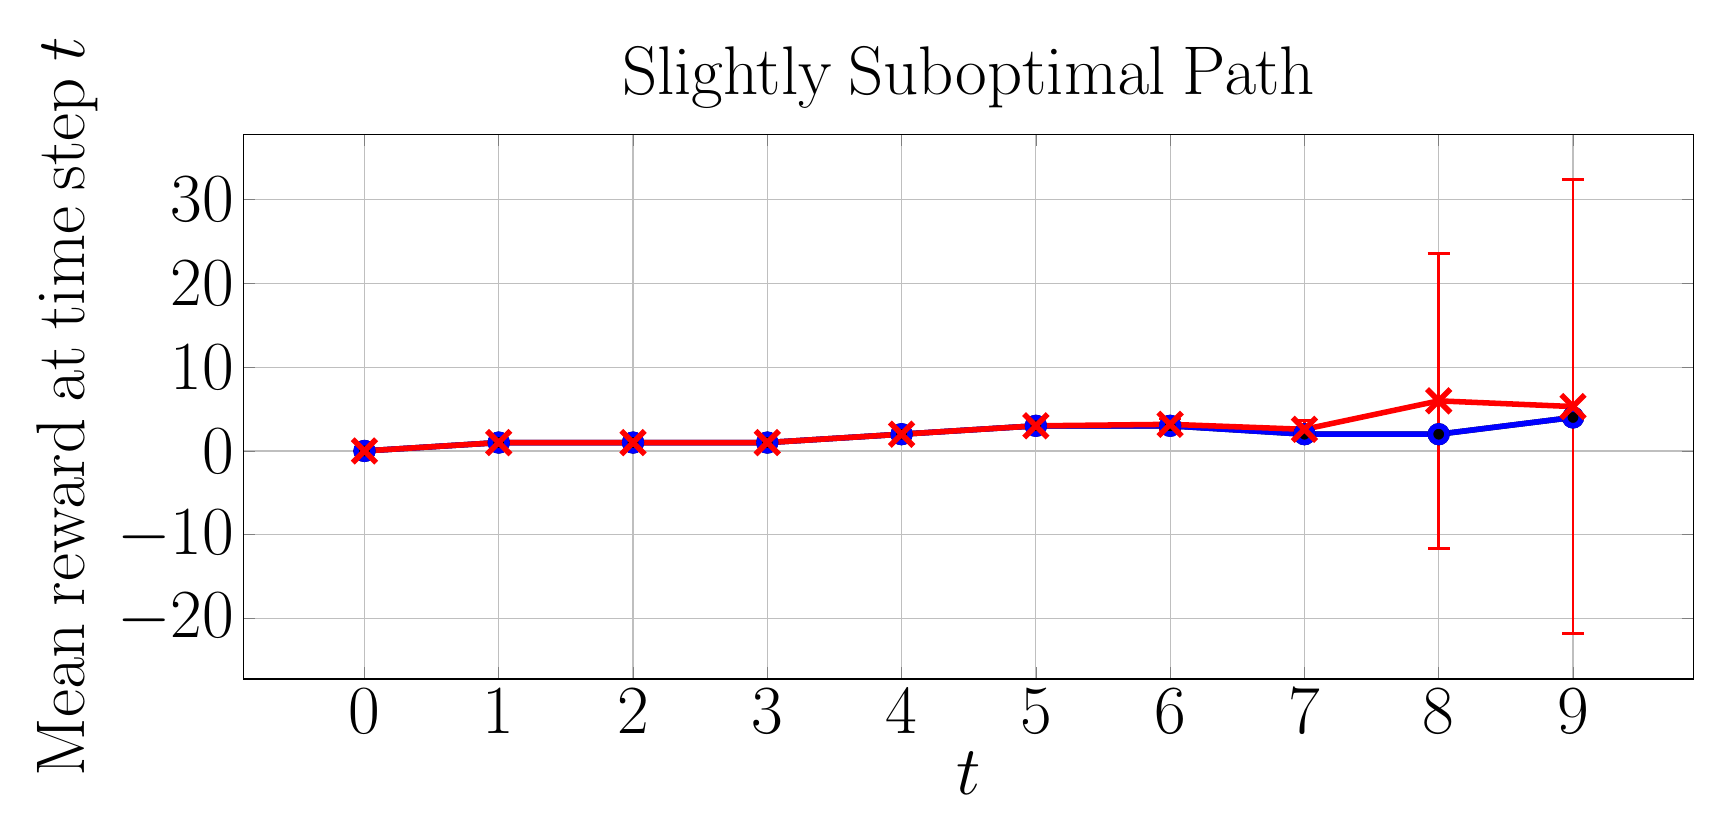
\begin{tikzpicture}
                \begin{axis}[
                    xlabel={$t$},
                    ylabel={Mean reward at time step $t$},
                    title={Slightly Suboptimal Path},
                    grid=both,
                    width=20cm, height=8.5cm,
                    every axis/.style={font=\Huge},
                    %
                ]
                \addplot[
                    color=black, %
                    mark=*, %
                    line width=2pt,
                    mark size=3pt,
                    error bars/.cd,
                    y dir=both, %
                    y explicit, %
                    error bar style={line width=1pt,solid},
                    error mark options={line width=1pt,mark size=4pt,rotate=90}
                ]
              coordinates {
                    (0, 0.0)  +- (0, 0.0)
                    (1, 1.0)  +- (0, 0.0) 
                    (2, 1.0)  +- (0, 0.0) 
                    (3, 1.0)  +- (0, 0.0)
                    (4, 2.0)  +- (0, 0.0)
                    (5, 3.0) +- (0, 0.0)
                    (6, 3.0) +- (0, 0.0)
                    (7, 2.0) +- (0, 0.0)
                    (8, 2.0) +- (0, 0.0)
                    (9, 4.0) +- (0, 0.0)
                };
                %
                \addplot[
                    color=blue, %
                    mark=o, %
                    line width=2pt,
                    mark size=3pt,
                    error bars/.cd,
                    y dir=both, %
                    y explicit, %
                    error bar style={line width=1pt,solid},
                    error mark options={line width=1pt,mark size=4pt,rotate=90}
                ]
              coordinates {
                    (0, 0.0)  +- (0, 0.0)
                    (1, 1.0)  +- (0, 0.0) 
                    (2, 1.0)  +- (0, 0.0) 
                    (3, 1.0)  +- (0, 0.0)
                    (4, 2.0)  +- (0, 0.0)
                    (5, 3.0) +- (0, 0.0)
                    (6, 3.0) +- (0, 0.0)
                    (7, 2.0) +- (0, 0.0)
                    (8, 2.0) +- (0, 0.0)
                    (9, 4.0) +- (0, 0.0)
                };
                %
                \addplot[
                    color=red, %
                    mark=x, %
                    line width=2pt,
                    mark size=6pt,
                    error bars/.cd,
                    y dir=both, %
                    y explicit, %
                    error bar style={line width=1pt,solid},
                    error mark options={line width=1pt,mark size=4pt,rotate=90}
                ]
                coordinates {
                    (0, 0.0)  +- (0, 0.0)
                    (1, 1.0)  +- (0, 0.0) 
                    (2, 1.0)  +- (0, 0.0) 
                    (3, 1.0)  +- (0, 0.0)
                    (4, 2.0)  += (0, 0.0)
                    (5, 3.0)  += (0, 0.0)
                    (6, 3.17847) += (0, 0.62606746) -= (0, 0.62606746)
                    (7, 2.5832885) += (0, 1.04598233) -= (0, 1.04598233)
                    (8, 5.978909) += (0, 17.60137623) -= (0, 17.60137623)
                    (9, 5.297059) += (0, 27.09227512) -= (0, 27.09227512)
                };
                \end{axis}
            \end{tikzpicture}
         }
    }\\[-1.5pt]
    \subfigure[\footnotesize Lowest cumulative reward: Interval CFMDP ($14$), Gumbel-max SCM ($-598$)]{%
         \resizebox{0.76\columnwidth}{!}{
             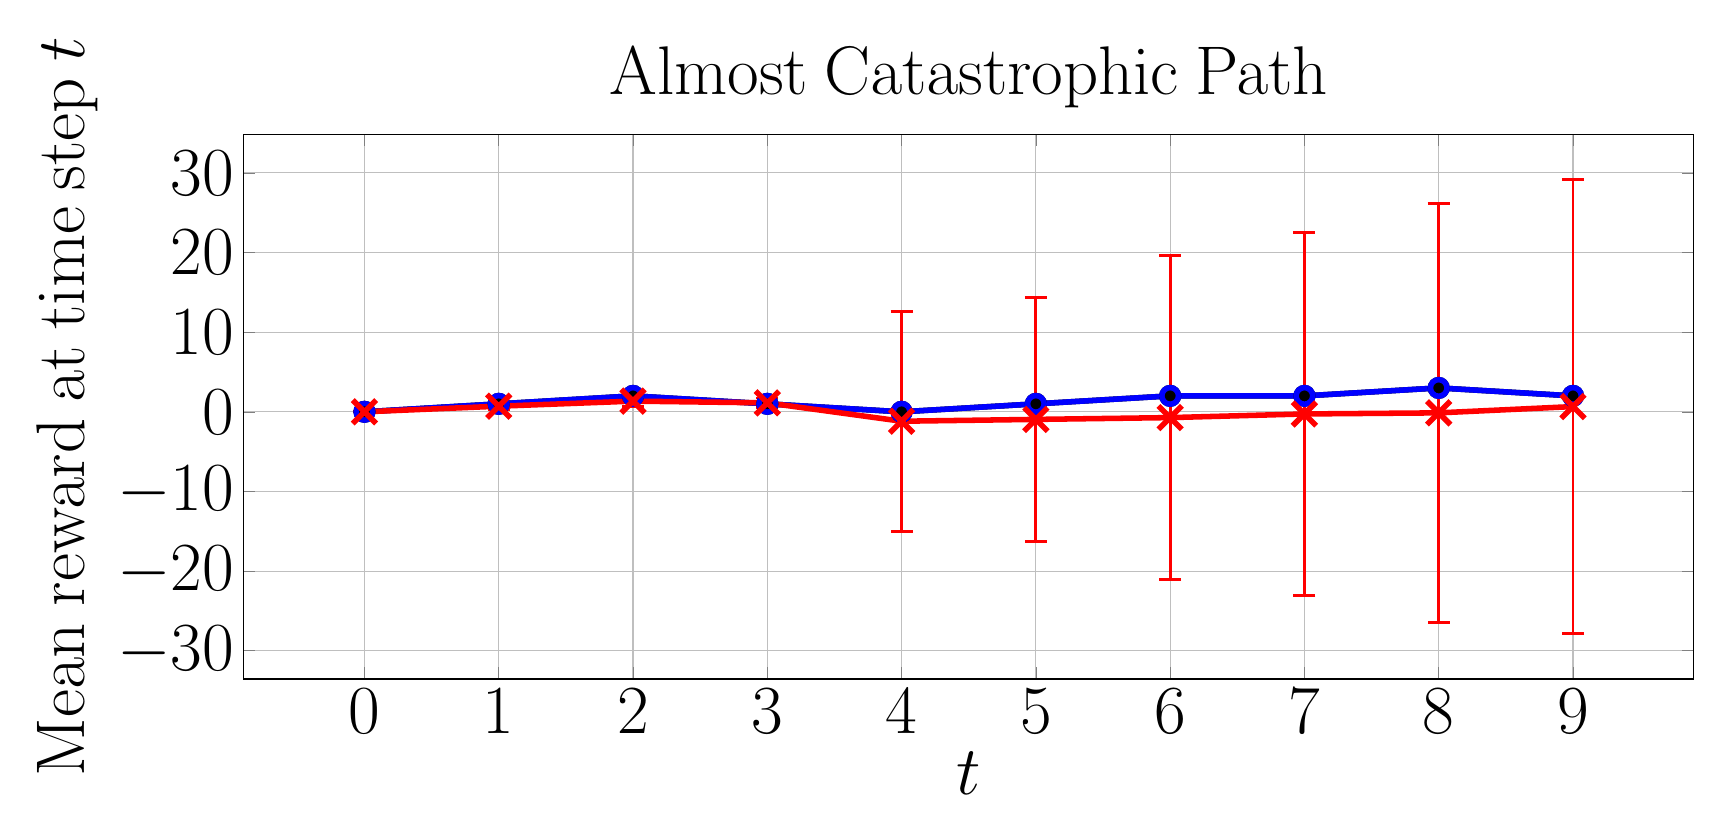
\begin{tikzpicture}
                \begin{axis}[
                    xlabel={$t$},
                    ylabel={Mean reward at time step $t$},
                    title={Almost Catastrophic Path},
                    grid=both,
                    width=20cm, height=8.5cm,
                    every axis/.style={font=\Huge},
                    %
                ]
                \addplot[
                    color=black, %
                    mark=*, %
                    line width=2pt,
                    mark size=3pt,
                    error bars/.cd,
                    y dir=both, %
                    y explicit, %
                    error bar style={line width=1pt,solid},
                    error mark options={line width=1pt,mark size=4pt,rotate=90}
                ]
                coordinates {
                    (0, 0.0)  +- (0, 0.0)
                    (1, 1.0)  +- (0, 0.0) 
                    (2, 2.0)  +- (0, 0.0) 
                    (3, 1.0)  +- (0, 0.0)
                    (4, 0.0)  +- (0, 0.0)
                    (5, 1.0) +- (0, 0.0)
                    (6, 2.0) +- (0, 0.0)
                    (7, 2.0) +- (0, 0.0)
                    (8, 3.0) +- (0, 0.0)
                    (9, 2.0) +- (0, 0.0)
                };
                %
                \addplot[
                    color=blue, %
                    mark=o, %
                    line width=2pt,
                    mark size=3pt,
                    error bars/.cd,
                    y dir=both, %
                    y explicit, %
                    error bar style={line width=1pt,solid},
                    error mark options={line width=1pt,mark size=4pt,rotate=90}
                ]
                coordinates {
                    (0, 0.0)  +- (0, 0.0)
                    (1, 1.0)  +- (0, 0.0) 
                    (2, 2.0)  +- (0, 0.0) 
                    (3, 1.0)  +- (0, 0.0)
                    (4, 0.0)  +- (0, 0.0)
                    (5, 1.0) +- (0, 0.0)
                    (6, 2.0) +- (0, 0.0)
                    (7, 2.0) +- (0, 0.0)
                    (8, 3.0) +- (0, 0.0)
                    (9, 2.0) +- (0, 0.0)
                };
                %
                \addplot[
                    color=red, %
                    mark=x, %
                    line width=2pt,
                    mark size=6pt,
                    error bars/.cd,
                    y dir=both, %
                    y explicit, %
                    error bar style={line width=1pt,solid},
                    error mark options={line width=1pt,mark size=4pt,rotate=90}
                ]
                coordinates {
                    (0, 0.0)  +- (0, 0.0)
                    (1, 0.7065655)  +- (0, 0.4553358) 
                    (2, 1.341673)  +- (0, 0.67091621) 
                    (3, 1.122926)  +- (0, 0.61281824)
                    (4, -1.1821935)  +- (0, 13.82444042)
                    (5, -0.952399)  +- (0, 15.35195457)
                    (6, -0.72672) +- (0, 20.33508414)
                    (7, -0.268983) +- (0, 22.77861454)
                    (8, -0.1310835) +- (0, 26.31013314)
                    (9, 0.65806) +- (0, 28.50670214)
                };
                %
            %
            %
            %
            %
            %
            %
            %
            %
            %
            %
            %
            %
            %
            %
            %
            %
            %
            %
                \end{axis}
            \end{tikzpicture}
         }
    }
    \hspace{1cm}
    \subfigure[\footnotesize Lowest cumulative reward: Interval CFMDP ($-698$), Gumbel-max SCM ($-698$)]{%
         \resizebox{0.76\columnwidth}{!}{
            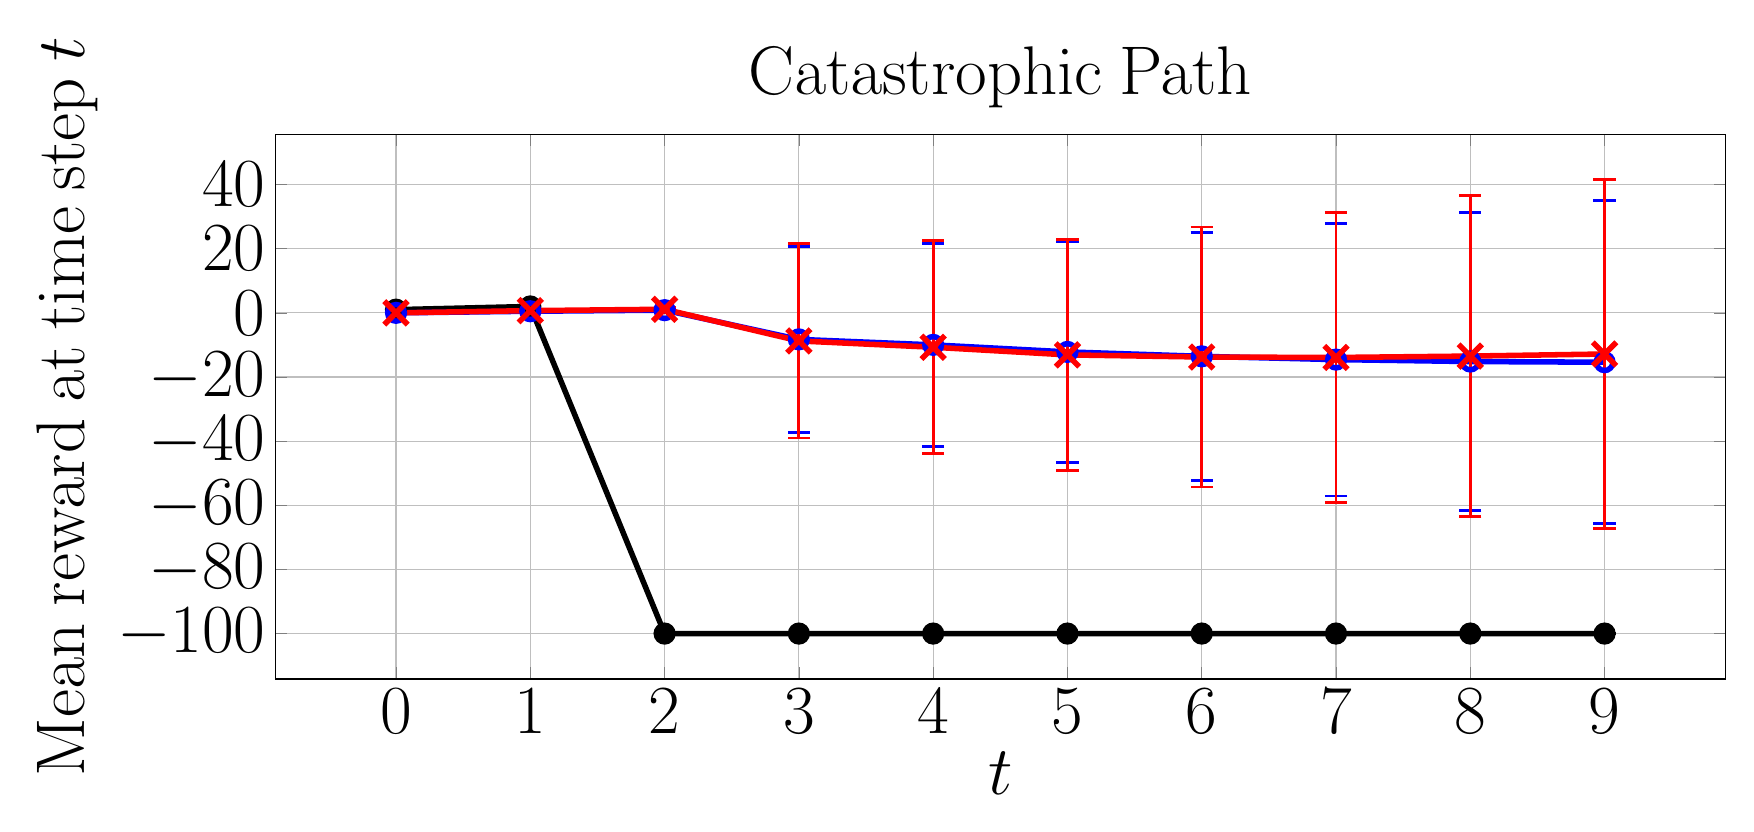
\begin{tikzpicture}
                \begin{axis}[
                    xlabel={$t$},
                    ylabel={Mean reward at time step $t$},
                    title={Catastrophic Path},
                    grid=both,
                    width=20cm, height=8.5cm,
                    every axis/.style={font=\Huge},
                    %
                ]
                \addplot[
                    color=black, %
                    mark=*, %
                    line width=2pt,
                    mark size=3pt,
                    error bars/.cd,
                    y dir=both, %
                    y explicit, %
                    error bar style={line width=1pt,solid},
                    error mark options={line width=1pt,mark size=4pt,rotate=90}
                ]
                coordinates {
                    (0, 1.0)  +- (0, 0.0)
                    (1, 2.0)  +- (0, 0.0) 
                    (2, -100.0)  +- (0, 0.0) 
                    (3, -100.0)  +- (0, 0.0)
                    (4, -100.0)  +- (0, 0.0)
                    (5, -100.0) +- (0, 0.0)
                    (6, -100.0) +- (0, 0.0)
                    (7, -100.0) +- (0, 0.0)
                    (8, -100.0) +- (0, 0.0)
                    (9, -100.0) +- (0, 0.0)
                };
                %
                \addplot[
                    color=blue, %
                    mark=o, %
                    line width=2pt,
                    mark size=3pt,
                    error bars/.cd,
                    y dir=both, %
                    y explicit, %
                    error bar style={line width=1pt,solid},
                    error mark options={line width=1pt,mark size=4pt,rotate=90}
                ]
                coordinates {
                    (0, 0.0)  +- (0, 0.0)
                    (1, 0.504814)  +- (0, 0.49997682) 
                    (2, 0.8439835)  +- (0, 0.76831917) 
                    (3, -8.2709165)  +- (0, 28.93656754)
                    (4, -9.981082)  +- (0, 31.66825363)
                    (5, -12.1776325) +- (0, 34.53463233)
                    (6, -13.556076) +- (0, 38.62845372)
                    (7, -14.574418) +- (0, 42.49603359)
                    (8, -15.1757075) +- (0, 46.41913968)
                    (9, -15.3900395) +- (0, 50.33563368)
                };
                %
                \addplot[
                    color=red, %
                    mark=x, %
                    line width=2pt,
                    mark size=6pt,
                    error bars/.cd,
                    y dir=both, %
                    y explicit, %
                    error bar style={line width=1pt,solid},
                    error mark options={line width=1pt,mark size=4pt,rotate=90}
                ]
                coordinates {
                    (0, 0.0)  +- (0, 0.0)
                    (1, 0.701873)  +- (0, 0.45743556) 
                    (2, 1.1227805)  +- (0, 0.73433129) 
                    (3, -8.7503255)  +- (0, 30.30257976)
                    (4, -10.722092)  +- (0, 33.17618589)
                    (5, -13.10721)  +- (0, 36.0648089)
                    (6, -13.7631645) +- (0, 40.56553451)
                    (7, -13.909043) +- (0, 45.23829402)
                    (8, -13.472517) +- (0, 49.96270296)
                    (9, -12.8278835) +- (0, 54.38618735)
                };
                %
            %
            %
            %
            %
            %
            %
            %
            %
            %
            %
            %
            %
            %
            %
            %
            %
            %
            %
                \end{axis}
            \end{tikzpicture}
         }
    }
    \caption{Average instant reward of CF paths induced by policies on GridWorld $p=0.4$.}
    \label{fig: reward p=0.4}
\end{figure*}

\subsection{Experimental Setup}
To compare policy performance, we measure the average rewards of counterfactual paths induced by our policy and the Gumbel-max policy by uniformly sampling $200$ counterfactual MDPs from the ICFMDP and generating $10,000$ counterfactual paths over each sampled CFMDP. \jl{Since the interval CFMDP depends on the observed path, we select $4$  paths of varying optimality to evaluate how the observed path impacts the performance of both policies: an optimal path, a slightly suboptimal path that could reach the optimal reward with a few changes, a catastrophic path that enters a catastrophic, terminal state with low reward, and an almost catastrophic path that was close to entering a catastrophic state.} When measuring the average probability bound widths and execution time needed to generate the ICFMDPs, we averaged over $20$ randomly generated observed paths
\footnote{Further training details are provided in Appendix \ref{app: training details}, and the code is provided at \href{https://github.com/ddv-lab/robust-cf-inference-in-MDPs}{https://github.com/ddv-lab/robust-cf-inference-in-MDPs}
%
%
.}.

\subsection{GridWorld}
\jl{The GridWorld MDP is a $4 \times 4$ grid where an agent must navigate from the top-left corner to the goal state in the bottom-right corner, avoiding a dangerous terminal state in the centre. At each time step, the agent can move up, down, left, or right, but there is a small probability (controlled by hyper-parameter $p$) of moving in an unintended direction. As the agent nears the goal, the reward for each state increases, culminating in a reward of $+100$ for reaching the goal. Entering the dangerous state results in a penalty of $-100$. We use two versions of GridWorld: a less stochastic version with $p=0.9$ (i.e., $90$\% chance of moving in the chosen direction) and a more stochastic version with $p=0.4$.}

\paragraph{GridWorld ($p=0.9$)}
When $p=0.9$, the counterfactual probability bounds are typically narrow (see Table \ref{tab:nonzero_probs} for average measurements). Consequently, as shown in Figure \ref{fig: reward p=0.9}, both policies are nearly identical and perform similarly well across the optimal, slightly suboptimal, and catastrophic paths.
%
However, for the almost catastrophic path, the interval CFMDP path is more conservative and follows the observed path more closely (as this is where the probability bounds are narrowest), which typically requires one additional step to reach the goal state than the Gumbel-max SCM policy.
%

\paragraph{GridWorld ($p=0.4$)}
\jl{When $p=0.4$, the GridWorld environment becomes more uncertain, increasing the risk of entering the dangerous state even if correct actions are chosen. Thus, as shown in Figure \ref{fig: reward p=0.4}, the interval CFMDP policy adopts a more conservative approach, avoiding deviation from the observed policy if it cannot guarantee higher counterfactual rewards (see the slightly suboptimal and almost catastrophic paths), whereas the Gumbel-max SCM is inconsistent: it can yield higher rewards, but also much lower rewards, reflected in the wide error bars.} For the catastrophic path, both policies must deviate from the observed path to achieve a higher reward and, in this case, perform similarly.
%
%
%
%
\subsection{Sepsis}
The Sepsis MDP \citep{oberst2019counterfactual} simulates trajectories of Sepsis patients. Each state consists of four vital signs (heart rate, blood pressure, oxygen concentration, and glucose levels), categorised as low, normal, or high.
and three treatments that can be toggled on/off at each time step (8 actions in total). Unlike \citet{oberst2019counterfactual}, we scale rewards based on the number of out-of-range vital signs, between $-1000$ (patient dies) and $1000$ (patient discharged). \jl{Like the GridWorld $p=0.4$ experiment, the Sepsis MDP is highly uncertain, as many states are equally likely to lead to optimal and poor outcomes. Thus, as shown in Figure \ref{fig: reward sepsis}, both policies follow the observed optimal and almost catastrophic paths to guarantee rewards are no worse than the observation.} However, improving the catastrophic path requires deviating from the observation. Here, the Gumbel-max SCM policy, on average, performs better than the interval CFMDP policy. But, since both policies have lower bounds clipped at $-1000$, neither policy reliably improves over the observation. In contrast, for the slightly suboptimal path, the interval CFMDP policy performs significantly better, shown by its higher lower bounds. 
Moreover, in these two cases, the worst-case counterfactual path generated by the interval CFMDP policy is better than that of the Gumbel-max SCM policy,
indicating its greater robustness.
%
\begin{figure*}
    \centering
     \resizebox{0.6\textwidth}{!}{
        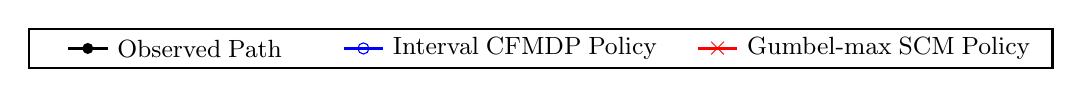
\begin{tikzpicture}[scale=1.0, every node/.style={scale=1.0}]
            \draw[thick, black] (-3, -0.25) rectangle (10, 0.25);
            %
            \draw[black, line width=1pt] (-2.5, 0.0) -- (-2,0.0);
            \fill[black] (-2.25,0.0) circle (2pt); %
            \node[right] at (-2,0.0) {\small Observed Path};
            
            %
            \draw[blue, line width=1pt] (1.0,0.0) -- (1.5,0.0);
            \node[draw=blue, circle, minimum size=4pt, inner sep=0pt] at (1.25,0.0) {}; %
            \node[right] at (1.5,0.0) {\small Interval CFMDP Policy};
            
            %
            \draw[red, line width=1pt] (5.5,0) -- (6,0);
            \node[red] at (5.75,0) {$\boldsymbol{\times}$}; %
            \node[right] at (6,0) {\small Gumbel-max SCM Policy};
        \end{tikzpicture}
    }\\
    \subfigure[\footnotesize Lowest cumulative reward: Interval CFMDP ($8000$), Gumbel-max SCM ($8000$)]{%
         \resizebox{0.76\columnwidth}{!}{
             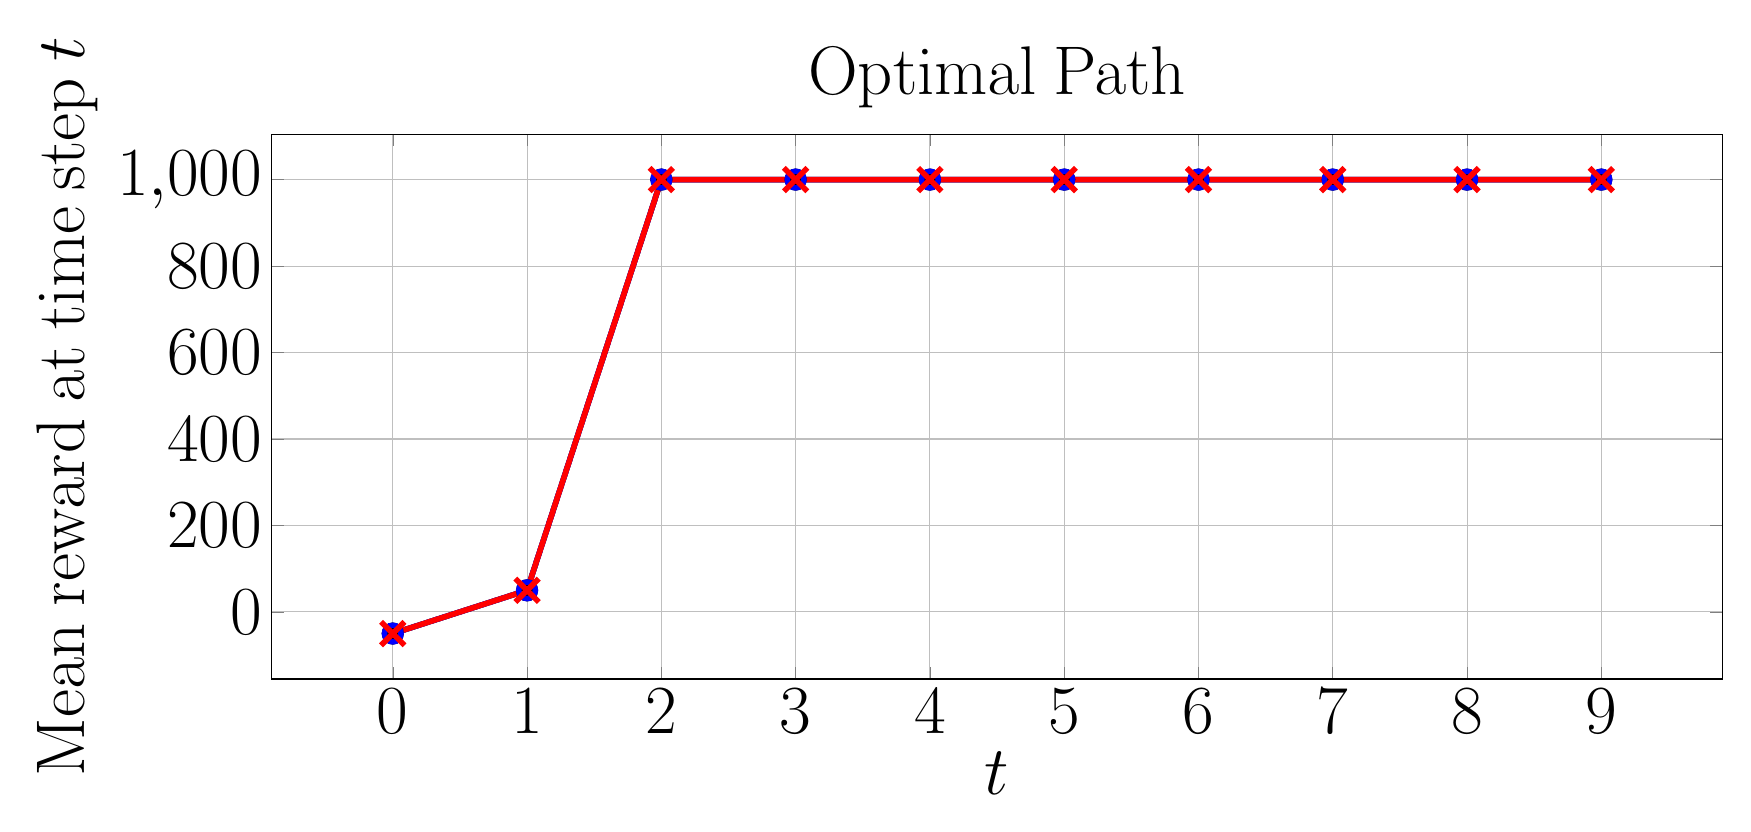
\begin{tikzpicture}
                \begin{axis}[
                    xlabel={$t$},
                    ylabel={Mean reward at time step $t$},
                    title={Optimal Path},
                    grid=both,
                    width=20cm, height=8.5cm,
                    every axis/.style={font=\Huge},
                    %
                ]
                \addplot[
                    color=black, %
                    mark=*, %
                    line width=2pt,
                    mark size=3pt,
                ]
                coordinates {
                    (0, -50.0)
                    (1, 50.0)
                    (2, 1000.0)
                    (3, 1000.0)
                    (4, 1000.0)
                    (5, 1000.0)
                    (6, 1000.0)
                    (7, 1000.0)
                    (8, 1000.0)
                    (9, 1000.0)
                };
                %
                \addplot[
                    color=blue, %
                    mark=o, %
                    line width=2pt,
                    mark size=3pt,
                    error bars/.cd,
                    y dir=both, %
                    y explicit, %
                    error bar style={line width=1pt,solid},
                    error mark options={line width=1pt,mark size=4pt,rotate=90}
                ]
                coordinates {
                    (0, -50.0)  +- (0, 0.0)
                    (1, 50.0)  +- (0, 0.0) 
                    (2, 1000.0)  +- (0, 0.0) 
                    (3, 1000.0)  +- (0, 0.0)
                    (4, 1000.0)  +- (0, 0.0)
                    (5, 1000.0) +- (0, 0.0)
                    (6, 1000.0) +- (0, 0.0)
                    (7, 1000.0) +- (0, 0.0)
                    (8, 1000.0) +- (0, 0.0)
                    (9, 1000.0) +- (0, 0.0)
                };
                %
                \addplot[
                    color=red, %
                    mark=x, %
                    line width=2pt,
                    mark size=6pt,
                    error bars/.cd,
                    y dir=both, %
                    y explicit, %
                    error bar style={line width=1pt,solid},
                    error mark options={line width=1pt,mark size=4pt,rotate=90}
                ]
                coordinates {
                    (0, -50.0)  +- (0, 0.0)
                    (1, 50.0)  +- (0, 0.0) 
                    (2, 1000.0)  +- (0, 0.0) 
                    (3, 1000.0)  +- (0, 0.0)
                    (4, 1000.0)  +- (0, 0.0)
                    (5, 1000.0) +- (0, 0.0)
                    (6, 1000.0) +- (0, 0.0)
                    (7, 1000.0) +- (0, 0.0)
                    (8, 1000.0) +- (0, 0.0)
                    (9, 1000.0) +- (0, 0.0)
                };
                %
                \end{axis}
            \end{tikzpicture}
         }
    }
    \hspace{1cm}
    \subfigure[\footnotesize Lowest cumulative reward: Interval CFMDP ($-5980$), Gumbel-max SCM ($-8000$)]{%
         \resizebox{0.76\columnwidth}{!}{
            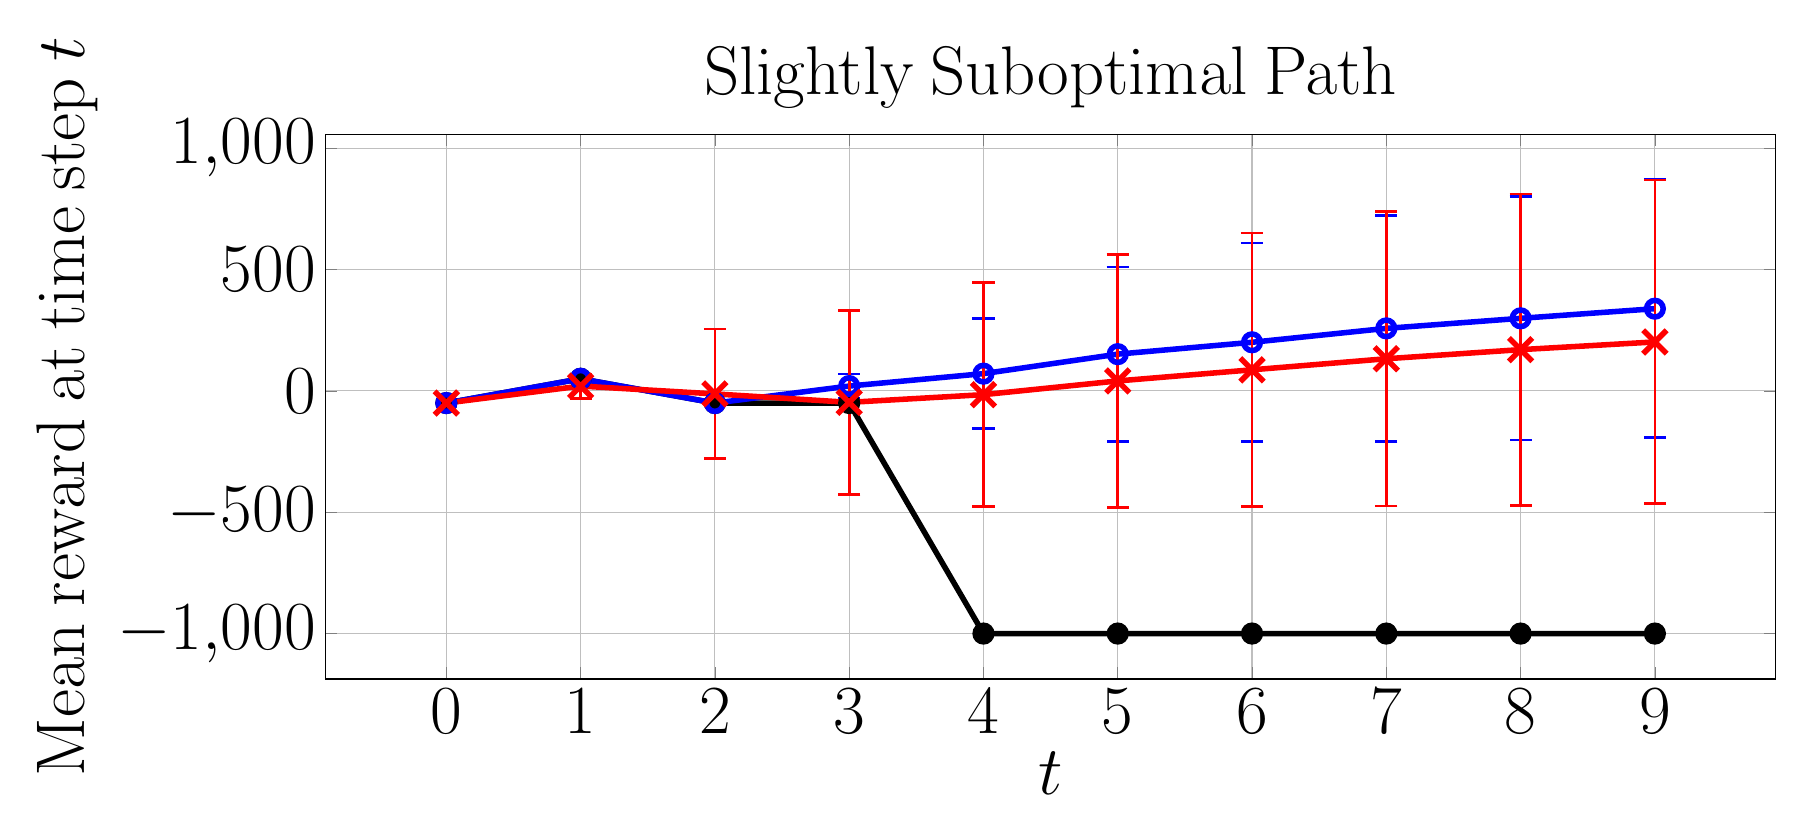
\begin{tikzpicture}
                \begin{axis}[
                    xlabel={$t$},
                    ylabel={Mean reward at time step $t$},
                    title={Slightly Suboptimal Path},
                    grid=both,
                    width=20cm, height=8.5cm,
                    every axis/.style={font=\Huge},
                    %
                ]
               \addplot[
                    color=black, %
                    mark=*, %
                    line width=2pt,
                    mark size=3pt,
                ]
                coordinates {
                    (0, -50.0)
                    (1, 50.0)
                    (2, -50.0)
                    (3, -50.0)
                    (4, -1000.0)
                    (5, -1000.0)
                    (6, -1000.0)
                    (7, -1000.0)
                    (8, -1000.0)
                    (9, -1000.0)
                };
                %
                \addplot[
                    color=blue, %
                    mark=o, %
                    line width=2pt,
                    mark size=3pt,
                    error bars/.cd,
                    y dir=both, %
                    y explicit, %
                    error bar style={line width=1pt,solid},
                    error mark options={line width=1pt,mark size=4pt,rotate=90}
                ]
                coordinates {
                    (0, -50.0)  +- (0, 0.0)
                    (1, 50.0)  +- (0, 0.0) 
                    (2, -50.0)  +- (0, 0.0) 
                    (3, 20.0631)  +- (0, 49.97539413)
                    (4, 71.206585)  +- (0, 226.02033693)
                    (5, 151.60797) +- (0, 359.23292559)
                    (6, 200.40593) +- (0, 408.86185176)
                    (7, 257.77948) +- (0, 466.10372804)
                    (8, 299.237465) +- (0, 501.82579506)
                    (9, 338.9129) +- (0, 532.06124996)
                };
                %
                \addplot[
                    color=red, %
                    mark=x, %
                    line width=2pt,
                    mark size=6pt,
                    error bars/.cd,
                    y dir=both, %
                    y explicit, %
                    error bar style={line width=1pt,solid},
                    error mark options={line width=1pt,mark size=4pt,rotate=90}
                ]
                coordinates {
                    (0, -50.0)  +- (0, 0.0)
                    (1, 20.00736)  +- (0, 49.99786741) 
                    (2, -12.282865)  +- (0, 267.598755) 
                    (3, -47.125995)  +- (0, 378.41755832)
                    (4, -15.381965)  +- (0, 461.77616558)
                    (5, 41.15459) +- (0, 521.53189262)
                    (6, 87.01595) +- (0, 564.22243126 )
                    (7, 132.62376) +- (0, 607.31338037)
                    (8, 170.168145) +- (0, 641.48013693)
                    (9, 201.813135) +- (0, 667.29441777)
                };
                %
                %
                %
                %
                %
                %
                %
                %
                %
                %
                %
                %
                %
                %
                %
                %
                %
                %
                %
                \end{axis}
            \end{tikzpicture}
         }
    }\\[-1.5pt]
    \subfigure[\footnotesize Lowest cumulative reward: Interval CFMDP ($100$), Gumbel-max SCM ($100$)]{%
         \resizebox{0.76\columnwidth}{!}{
             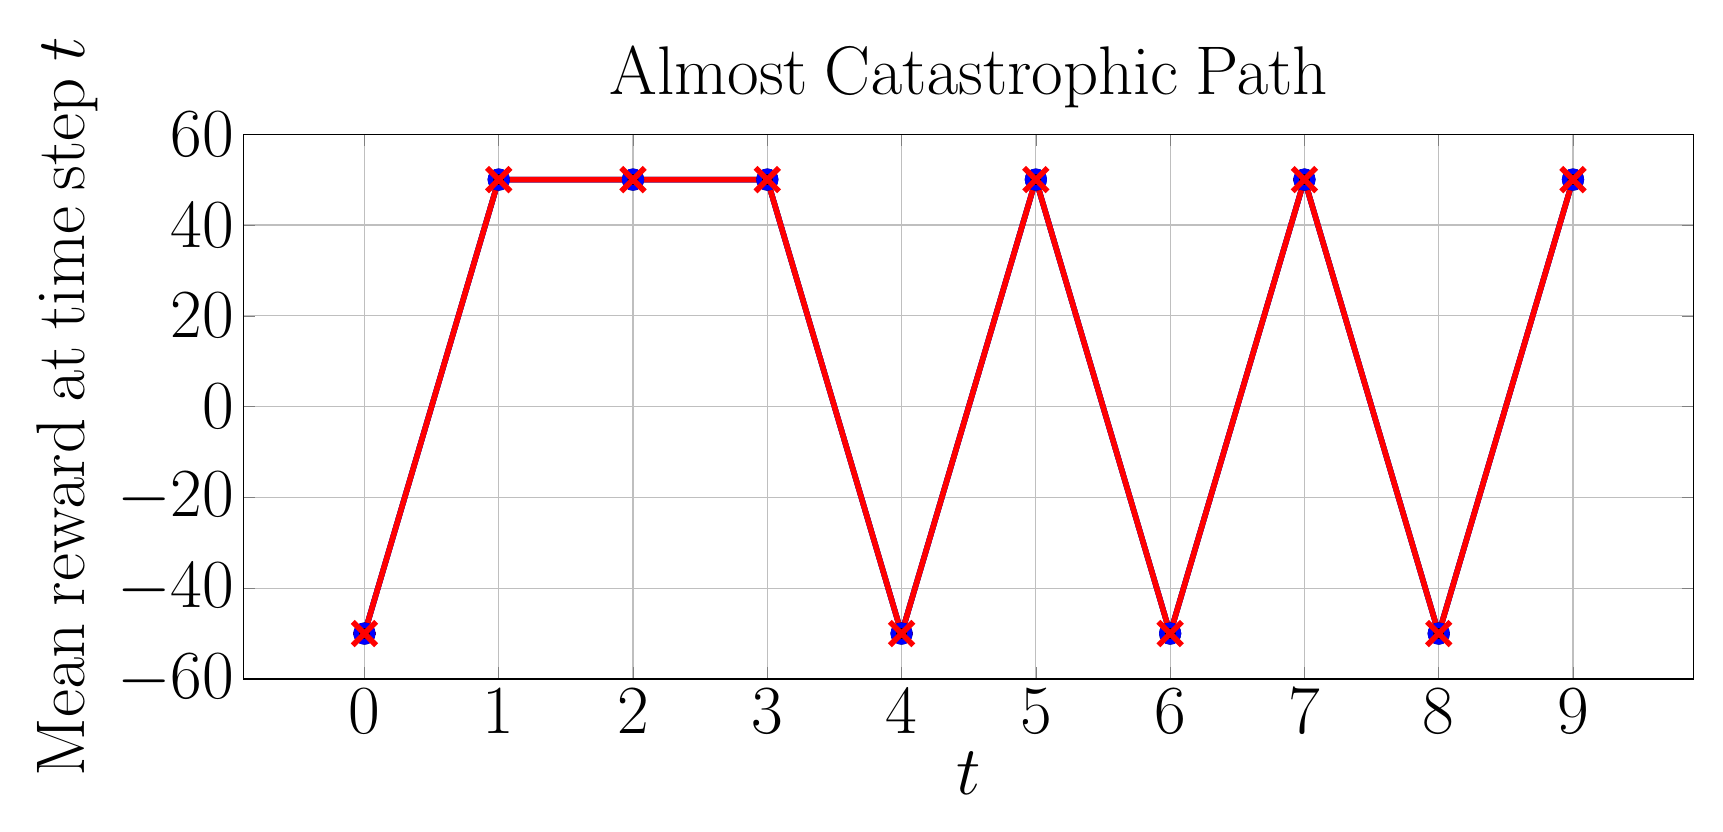
\begin{tikzpicture}
                \begin{axis}[
                    xlabel={$t$},
                    ylabel={Mean reward at time step $t$},
                    title={Almost Catastrophic Path},
                    grid=both,
                    every axis/.style={font=\Huge},
                    width=20cm, height=8.5cm,
                    %
                ]
               \addplot[
                    color=black, %
                    mark=*, %
                    line width=2pt,
                    mark size=3pt,
                ]
                coordinates {
                    (0, -50.0)
                    (1, 50.0)
                    (2, 50.0)
                    (3, 50.0)
                    (4, -50.0)
                    (5, 50.0)
                    (6, -50.0)
                    (7, 50.0)
                    (8, -50.0)
                    (9, 50.0)
                };
                %
                %
                \addplot[
                    color=blue, %
                    mark=o, %
                    line width=2pt,
                    mark size=3pt,
                    error bars/.cd,
                    y dir=both, %
                    y explicit, %
                    error bar style={line width=1pt,solid},
                    error mark options={line width=1pt,mark size=4pt,rotate=90}
                ]
                coordinates {
                    (0, -50.0)  +- (0, 0.0)
                    (1, 50.0)  +- (0, 0.0) 
                    (2, 50.0)  +- (0, 0.0) 
                    (3, 50.0)  +- (0, 0.0)
                    (4, -50.0)  +- (0, 0.0)
                    (5, 50.0) +- (0, 0.0)
                    (6, -50.0) +- (0, 0.0)
                    (7, 50.0) +- (0, 0.0)
                    (8, -50.0) +- (0, 0.0)
                    (9, 50.0) +- (0, 0.0)
                };
                %
                \addplot[
                    color=red, %
                    mark=x, %
                    line width=2pt,
                    mark size=6pt,
                    error bars/.cd,
                    y dir=both, %
                    y explicit, %
                    error bar style={line width=1pt,solid},
                    error mark options={line width=1pt,mark size=4pt,rotate=90}
                ]
                coordinates {
                    (0, -50.0)  +- (0, 0.0)
                    (1, 50.0)  +- (0, 0.0) 
                    (2, 50.0)  +- (0, 0.0) 
                    (3, 50.0)  +- (0, 0.0)
                    (4, -50.0)  +- (0, 0.0)
                    (5, 50.0) +- (0, 0.0)
                    (6, -50.0) +- (0, 0.0)
                    (7, 50.0) +- (0, 0.0)
                    (8, -50.0) +- (0, 0.0)
                    (9, 50.0) +- (0, 0.0)
                };
                %
                %
                %
                %
                %
                %
                %
                %
                %
                %
                %
                %
                %
                %
                %
                %
                %
                %
                %
                \end{axis}
            \end{tikzpicture}
         }
    }
    \hspace{1cm}
    \subfigure[\footnotesize Lowest cumulative reward: Interval CFMDP ($-7150$), Gumbel-max SCM ($-9050$)]{%
         \resizebox{0.76\columnwidth}{!}{
            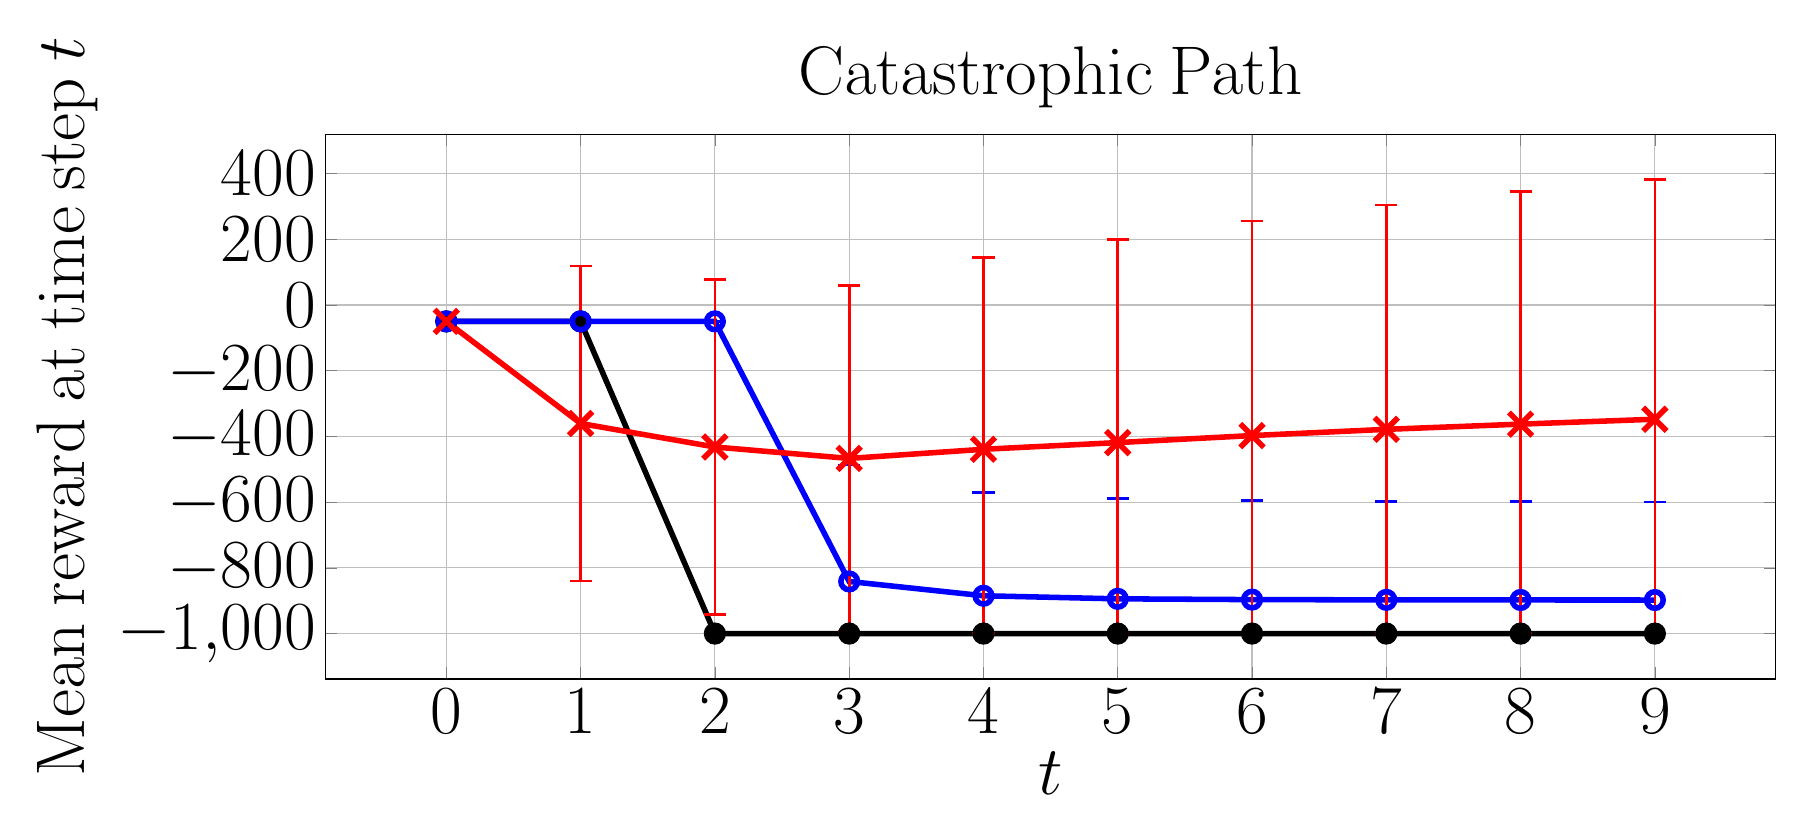
\begin{tikzpicture}
                \begin{axis}[
                    xlabel={$t$},
                    ylabel={Mean reward at time step $t$},
                    title={Catastrophic Path},
                    grid=both,
                    width=20cm, height=8.5cm,
                    every axis/.style={font=\Huge},
                    %
                ]
               \addplot[
                    color=black, %
                    mark=*, %
                    line width=2pt,
                    mark size=3pt,
                ]
                coordinates {
                    (0, -50.0)
                    (1, -50.0)
                    (2, -1000.0)
                    (3, -1000.0)
                    (4, -1000.0)
                    (5, -1000.0)
                    (6, -1000.0)
                    (7, -1000.0)
                    (8, -1000.0)
                    (9, -1000.0)
                };
                %
                %
                \addplot[
                    color=blue, %
                    mark=o, %
                    line width=2pt,
                    mark size=3pt,
                    error bars/.cd,
                    y dir=both, %
                    y explicit, %
                    error bar style={line width=1pt,solid},
                    error mark options={line width=1pt,mark size=4pt,rotate=90}
                ]
                coordinates {
                    (0, -50.0)  +- (0, 0.0)
                    (1, -50.0)  +- (0, 0.0) 
                    (2, -50.0)  +- (0, 0.0) 
                    (3, -841.440725)  += (0, 354.24605512) -= (0, 158.559275)
                    (4, -884.98225)  += (0, 315.37519669) -= (0, 115.01775)
                    (5, -894.330425) += (0, 304.88572805) -= (0, 105.669575)
                    (6, -896.696175) += (0, 301.19954514) -= (0, 103.303825)
                    (7, -897.4635) += (0, 299.61791279) -= (0, 102.5365)
                    (8, -897.77595) += (0, 298.80392585) -= (0, 102.22405)
                    (9, -897.942975) += (0, 298.32920557) -= (0, 102.057025)
                };
                %
                \addplot[
                    color=red, %
                    mark=x, %
                    line width=2pt,
                    mark size=6pt,
                    error bars/.cd,
                    y dir=both, %
                    y explicit, %
                    error bar style={line width=1pt,solid},
                    error mark options={line width=1pt,mark size=4pt,rotate=90}
                ]
            coordinates {
                    (0, -50.0)  +- (0, 0.0)
                    (1, -360.675265)  +- (0, 479.39812699) 
                    (2, -432.27629)  +- (0, 510.38620897) 
                    (3, -467.029545)  += (0, 526.36009628) -= (0, 526.36009628)
                    (4, -439.17429)  += (0, 583.96638919) -= (0, 560.82571)
                    (5, -418.82704) += (0, 618.43027478) -= (0, 581.17296)
                    (6, -397.464895) += (0, 652.67322574) -= (0, 602.535105)
                    (7, -378.49052) += (0, 682.85407033) -= (0, 621.50948)
                    (8, -362.654195) += (0, 707.01412023) -= (0, 637.345805)
                    (9, -347.737935) += (0, 729.29076479) -= (0, 652.262065)
                };
                %
                %
                %
                %
                %
                %
                %
                %
                %
                %
                %
                %
                %
                %
                %
                %
                %
                %
                %
                \end{axis}
            \end{tikzpicture}
         }
    }
    \caption{Average instant reward of CF paths induced by policies on Sepsis.}
    \label{fig: reward sepsis}
\end{figure*}

%
%
%
\subsection{Interval CFMDP Bounds}
%
%
Table \ref{tab:nonzero_probs} presents the mean counterfactual probability bound widths (excluding transitions where the upper bound is $0$) for each MDP, averaged over 20 observed paths. We compare the bounds under counterfactual stability (CS) and monotonicity (M) assumptions, CS alone, and no assumptions. This shows that the assumptions marginally reduce the bound widths, indicating the assumptions tighten the bounds without excluding too many causal models, as intended.
\renewcommand{\arraystretch}{1}

\begin{table}
\centering
\caption{Mean width of counterfactual probability bounds}
\resizebox{0.8\columnwidth}{!}{%
\begin{tabular}{|c|c|c|c|}
\hline
\multirow{2}{*}{\textbf{Environment}} & \multicolumn{3}{c|}{\textbf{Assumptions}} \\ \cline{2-4}
 & \textbf{CS + M} & \textbf{CS} & \textbf{None\tablefootnote{\jl{Equivalent to \citet{li2024probabilities}'s bounds (see Section \ref{sec: equivalence with Li}).}}} \\ \hline
\textbf{GridWorld} ($p=0.9$) & 0.0817 & 0.0977 & 0.100 \\ \hline
\textbf{GridWorld} ($p=0.4$) & 0.552  & 0.638  & 0.646 \\ \hline
\textbf{Sepsis} & 0.138 & 0.140 & 0.140 \\ \hline
\end{tabular}
}
\label{tab:nonzero_probs}
\end{table}


\subsection{Execution Times}
Table \ref{tab: times} compares the average time needed to generate the interval CFMDP vs.\ the Gumbel-max SCM CFMDP for 20 observations.
The GridWorld algorithms were run single-threaded, while the Sepsis experiments were run in parallel.
Generating the interval CFMDP is significantly faster as it uses exact analytical bounds, whereas the Gumbel-max CFMDP requires sampling from the Gumbel distribution to estimate counterfactual transition probabilities. \jl{Since constructing the counterfactual MDP models is the main bottleneck in both approaches, ours is more efficient overall and suitable for larger MDPs.}
\begin{table}
\centering
\caption{Mean execution time to generate CFMDPs}
\resizebox{0.99\columnwidth}{!}{%
\begin{tabular}{|c|c|c|}
\hline
\multirow{2}{*}{\textbf{Environment}} & \multicolumn{2}{c|}{\textbf{Mean Execution Time (s)}} \\ \cline{2-3} 
                                      & \textbf{Interval CFMDP} & \textbf{Gumbel-max CFMDP} \\ \hline
\textbf{GridWorld ($p=0.9$) }                  & 0.261                   & 56.1                      \\ \hline
\textbf{GridWorld ($p=0.4$)  }                 & 0.336                   & 54.5                      \\ \hline
\textbf{Sepsis}                                 & 688                     & 2940                      \\ \hline
\end{tabular}%
}
\label{tab: times}
\end{table}

\section{Related Work}
The landscape of large language model vulnerabilities has been extensively studied in recent literature \cite{crothers2023machinegeneratedtextcomprehensive,shayegani2023surveyvulnerabilitieslargelanguage,Yao_2024,Huang2023ASO}, that propose detailed taxonomies of threats. These works categorize LLM attacks into distinct types, such as adversarial attacks, data poisoning, and specific vulnerabilities related to prompt engineering. Among these, prompt injection attacks have emerged as a significant and distinct category, underscoring their relevance to LLM security.

The following high-level overview of the collected taxonomy of LLM vulnerabilities is defined in \cite{Yao_2024}:
\begin{itemize}
    \item Adversarial Attacks: Data Poisoning, Backdoor Attacks
    \item Inference Attacks: Attribute Inference, Membership Inferences
    \item Extraction Attacks
    \item Bias and Unfairness
Exploitation
    \item Instruction Tuning Attacks: Jailbreaking, Prompt Injection.
\end{itemize}
Prompt injection attacks are further classified in \cite{shayegani2023surveyvulnerabilitieslargelanguage} into the following: Goal hijacking and \textbf{Prompt leakage}.

The reviewed taxonomies underscore the need for comprehensive frameworks to evaluate LLM security. The agentic approach introduced in this paper builds on these insights, automating adversarial testing to address a wide range of scenarios, including those involving prompt leakage and role-specific vulnerabilities.

\subsection{Prompt Injection and Prompt Leakage}

Prompt injection attacks exploit the blending of instructional and data inputs, manipulating LLMs into deviating from their intended behavior. Prompt injection attacks encompass techniques that override initial instructions, expose private prompts, or generate malicious outputs \cite{Huang2023ASO}. A subset of these attacks, known as prompt leakage, aims specifically at extracting sensitive system prompts embedded within LLM configurations. In \cite{shayegani2023surveyvulnerabilitieslargelanguage}, authors differentiate between prompt leakage and related methods such as goal hijacking, further refining the taxonomy of LLM-specific vulnerabilities.

\subsection{Defense Mechanisms}

Various defense mechanisms have been proposed to address LLM vulnerabilities, particularly prompt injection and leakage \cite{shayegani2023surveyvulnerabilitieslargelanguage,Yao_2024}. We focused on cost-effective methods like instruction postprocessing and prompt engineering, which are viable for proprietary models that cannot be retrained. Instruction preprocessing sanitizes inputs, while postprocessing removes harmful outputs, forming a dual-layer defense. Preprocessing methods include perplexity-based filtering \cite{Jain2023BaselineDF,Xu2022ExploringTU} and token-level analysis \cite{Kumar2023CertifyingLS}. Postprocessing employs another set of techniques, such as censorship by LLMs \cite{Helbling2023LLMSD,Inan2023LlamaGL}, and use of canary tokens and pattern matching \cite{vigil-llm,rebuff}, although their fundamental limitations are noted \cite{Glukhov2023LLMCA}. Prompt engineering employs carefully designed instructions \cite{Schulhoff2024ThePR} and advanced techniques like spotlighting \cite{Hines2024DefendingAI} to mitigate vulnerabilities, though no method is foolproof \cite{schulhoff-etal-2023-ignore}. Adversarial training, by incorporating adversarial examples into the training process, strengthens models against attacks \cite{Bespalov2024TowardsBA,Shaham2015UnderstandingAT}.

\subsection{Security Testing for Prompt Injection Attacks}

Manual testing, such as red teaming \cite{ganguli2022redteaminglanguagemodels} and handcrafted "Ignore Previous Prompt" attacks \cite{Perez2022IgnorePP}, highlights vulnerabilities but is limited in scale. Automated approaches like PAIR \cite{chao2024jailbreakingblackboxlarge} and GPTFUZZER \cite{Yu2023GPTFUZZERRT} achieve higher success rates by refining prompts iteratively or via automated fuzzing. Red teaming with LLMs \cite{Perez2022RedTL} and reinforcement learning \cite{anonymous2024diverse} uncovers diverse vulnerabilities, including data leakage and offensive outputs. Indirect Prompt Injection (IPI) manipulates external data to compromise applications \cite{Greshake2023NotWY}, adapting techniques like SQL injection to LLMs \cite{Liu2023PromptIA}. Prompt secrecy remains fragile, with studies showing reliable prompt extraction \cite{Zhang2023EffectivePE}. Advanced frameworks like Token Space Projection \cite{Maus2023AdversarialPF} and Weak-to-Strong Jailbreaking Attacks \cite{zhao2024weaktostrongjailbreakinglargelanguage} exploit token-space relationships, achieving high success rates for prompt extraction and jailbreaking.

\subsection{Agentic Frameworks for Evaluating LLM Security}

The development of multi-agent systems leveraging large language models (LLMs) has shown promising results in enhancing task-solving capabilities \cite{Hong2023MetaGPTMP, Wang2023UnleashingTE, Talebirad2023MultiAgentCH, Wu2023AutoGenEN, Du2023ImprovingFA}. A key aspect across various frameworks is the specialization of roles among agents \cite{Hong2023MetaGPTMP, Wu2023AutoGenEN}, which mimics human collaboration and improves task decomposition.

Agentic frameworks and the multi-agent debate approach benefit from agent interaction, where agents engage in conversations or debates to refine outputs and correct errors \cite{Wu2023AutoGenEN}. For example, debate systems improve factual accuracy and reasoning by iteratively refining responses through collaborative reasoning \cite{Du2023ImprovingFA}, while AG2 allows agents to autonomously interact and execute tasks with minimal human input.

These frameworks highlight the viability of agentic systems, showing how specialized roles and collaborative mechanisms lead to improved performance, whether in factuality, reasoning, or task execution. By leveraging the strengths of diverse agents, these systems demonstrate a scalable approach to problem-solving.

Recent research on testing LLMs using other LLMs has shown that this approach can be highly effective \cite{chao2024jailbreakingblackboxlarge, Yu2023GPTFUZZERRT, Perez2022RedTL}. Although the papers do not explicitly employ agentic frameworks they inherently reflect a pattern similar to that of an "attacker" and a "judge". \cite{chao2024jailbreakingblackboxlarge}  This pattern became a focal point for our work, where we put the judge into a more direct dialogue, enabling it to generate attacks based on the tested agent response in an active conversation.

A particularly influential paper in shaping our approach is Jailbreaking Black Box Large Language Models in Twenty Queries \cite{chao2024jailbreakingblackboxlarge}. This paper not only introduced the attacker/judge architecture but also provided the initial system prompts used for a judge.
\section{Conclusion}
In this work, we propose a simple yet effective approach, called SMILE, for graph few-shot learning with fewer tasks. Specifically, we introduce a novel dual-level mixup strategy, including within-task and across-task mixup, for enriching the diversity of nodes within each task and the diversity of tasks. Also, we incorporate the degree-based prior information to learn expressive node embeddings. Theoretically, we prove that SMILE effectively enhances the model's generalization performance. Empirically, we conduct extensive experiments on multiple benchmarks and the results suggest that SMILE significantly outperforms other baselines, including both in-domain and cross-domain few-shot settings.

\section*{Acknowledgments}
This work is supported in part by the National Science Foundation under award numbers 1900654, 1956393, 2339266, and a gift from the UC Noyce Foundation. We would like to thank Muhammad Haroon, Shraddha Hardikar, and Luca Baldesi, for their preliminary assistance and feedback on how \autolike{} can be implemented and evaluated. 
 



\bibliographystyle{ACM-Reference-Format}
\bibliography{master,online}


\appendix
\section{Ethical Considerations}
\label{app:ethics}
In this work, we discuss sensitive topics and issues, such as mental health, eating disorders, and self-harm. All of the experiments in Sec.~\ref{sec:autolike-prelim-results} were automated and did not involve any real human users. Manual evaluation of sensitive materials was completed by the authors, who provided  expressed consent and affirmed to the team that they were not adversely affected by the review process. Furthermore, our implementation and deployment of \autolike{} on TikTok aimed to reduce its impact on the platform. For instance, our implementation automatically skipped TikTok ads. In addition, the streamlined design of \autolike{} in Sec.~\ref{sec:tiktok-eval} reduced the amount of TikToks processed from potential tens of thousands down to 200 TikToks per experiment. Similarly, we designed the controlled experiment to be re-usable, which further minimized the impact on TikTok.

\end{document}
